 
\documentclass[12pt]{article}
 %author David Dobor
\usepackage[margin=1in]{geometry} 
\usepackage{amsmath,amsthm,amssymb}
 \usepackage{graphicx}
 \usepackage{multirow}
\usepackage[scaled]{helvet}
\usepackage{hyperref}
\usepackage[usenames,dvipsnames,svgnames,table]{xcolor}
\usepackage[T1]{fontenc}
\usepackage{palatino}
\usepackage{enumerate}
%\renewcommand*\familydefault{\sfdefault} %% Only if the base font of the document is to be sans serif

%listings package for formatting code
%\usepackage{listings}


\newcommand{\N}{\mathbb{N}}
\newcommand{\Z}{\mathbb{Z}}


\newcommand{\blditA}{\textbf{\textit{A}}}
\newcommand{\blditB}{\textbf{\textit{B}}}
\newcommand{\blditC}{\textbf{\textit{C}}}
\newcommand{\blditP}{\textbf{\textit{P}}}
\newcommand{\blditQ}{\textbf{\textit{Q}}}
\newcommand{\bldI}{\textbf{I}}
\newcommand{\blditX}{\textbf{\textit{X}}}
 
\newenvironment{theorem}[2][Theorem]{\begin{trivlist}
\item[\hskip \labelsep {\bfseries #1}\hskip \labelsep {\bfseries #2.}]}{\end{trivlist}}
\newenvironment{lemma}[2][Lemma]{\begin{trivlist}
\item[\hskip \labelsep {\bfseries #1}\hskip \labelsep {\bfseries #2.}]}{\end{trivlist}}
\newenvironment{exercise}[2][Exercise]{\begin{trivlist}
\item[\hskip \labelsep {\bfseries #1}\hskip \labelsep {\bfseries #2.}]}{\end{trivlist}}
\newenvironment{problem}[2][Problem]{\begin{trivlist}
\item[\hskip \labelsep {\bfseries #1}\hskip \labelsep {\bfseries #2.}]}{\end{trivlist}}
\newenvironment{question}[2][Question]{\begin{trivlist}
\item[\hskip \labelsep {\bfseries #1}\hskip \labelsep {\bfseries #2.}]}{\end{trivlist}}
\newenvironment{answer}[2][Answer]{\begin{trivlist}
\item[\hskip \labelsep {\bfseries #1}\hskip \labelsep {\bfseries #2.}]}{\end{trivlist}}

\begin{document}
 \renewcommand{\arraystretch}{1.3}

 
\title{Stat 8003, Homework 3}%replace X with the appropriate number
\author{Group G: Andrew Schneider,  Abdulsalam Hdadi, David Dobor
\\ %replace with your name
} %if necessary, replace with your course title
 
\maketitle
 
 %%%%%%%% Question 1 %%%%%%%%%
 
\begin{question}{3.1} %You can use theorem, exercise, problem, or question here.  Modify 1.1to be whatever number you are proving
Consider a bivariate distribution with $P(X = 1,Y = 2) = 0.4, P(X = 2,Y = 3) = 0.6.$ Find the correlation coefficient between $X$ and $Y$.
\end{question}
 
 \textbf{\color{TealBlue}\emph{Answer:} } 
We fill the following table with the given joint probability density. (If  $X$ and $Y$ attain other values, the joint density at those values must be zero, since the given probabilities already sum up to 1.) The marginal probabilities are given at the right and at the bottom margins of the table. All entries in the joint table sum up to 1; the entries in the margins also sum up to 1:


\bigskip
\begin{center}
\begin{tabular}{ r c c c}
\multicolumn{1}{r}{}
 &  \multicolumn{1}{c}{$X = 1$}
 & \multicolumn{1}{c}{$X = 2$} 
 & \multicolumn{1}{c} {$P(Y = y):$}\\
\cline{2-3}
$Y = 2$ & \multicolumn{1}{|c|}{$2/5$ } & \multicolumn{1}{c|}{$0$ }  & \emph{2/5}\\
\cline{2-3}
$Y = 3$ & \multicolumn{1}{|c|}{$0$}  & \multicolumn{1}{c|}{$3/5$} & \emph{3/5}\\ 
\cline{2-3}

\cline{4-4}
$P(X = x):$ & \emph{2/5} & \multicolumn{1}{c|}{\emph{3/5}}  & \multicolumn{1}{c|}{\textbf{\textit{1}}}\\
\cline{4-4}
\end{tabular}
 \end{center}

\bigskip
 
 The correlation coefficient here is $1$. We verify this by direct computation:

\begin{align*}
E[X] = 1 \cdot \frac{2}{5} +  2 \cdot \frac{3}{5} = \frac{8}{5}        \\
E[X^2] = 1^2 \cdot  \frac{2}{5} +  2^2 \cdot \frac{3}{5} = \frac{14}{5}  \\
Var(X) = E[X^2]  - (E[X])^2 =  \frac{14}{5} - \left(\frac{8}{5} \right)^2 = \frac{6}{25}
\end{align*}


\begin{align*}
E[Y] = 2 \cdot \frac{2}{5} +  3 \cdot \frac{3}{5} = \frac{13}{5}        \\
E[Y^2] = 2^2 \cdot  \frac{2}{5} +  3^2 \cdot \frac{3}{5} = 7  \\
Var(Y) = E[Y^2]  - (E[X])^2 =  7 - \left(\frac{13}{5} \right)^2 = \frac{6}{25}
\end{align*}
 

\begin{align*}
E[XY] = 1 \cdot 2 \cdot \frac{2}{5} +  2 \cdot 3 \cdot \frac{3}{5} = \frac{22}{5}        \\
E[X] \cdot E[Y] = \frac{8}{5} \cdot \frac{13}{5} = \frac{104}{25}  \\
Cov(X,Y) = E[XY] - E[X] \cdot E[Y] = \frac{22}{5}  -  \frac{104}{25} = \frac{6}{25}
\end{align*}

Therefore, the correlation coefficiant is:

$$
\rho = \frac{Cov(X,Y)} {\sqrt{ Var(X) \cdot Var(Y) }} = \frac{6/25} {\sqrt{6/25 \cdot 6/25}} = 1
$$


\bigskip
\bigskip
 %%%%%%%% Question 2 %%%%%%%%%
\begin{question}{3.2}

Find two random variables $X$ and $Y$ , such that $Cov(X, Y ) = 0$ but $X$ and $Y$ are not independent.

\end{question}

 \textbf{\color{TealBlue}\emph{Answer:} } 
Let $X$ be Bernoulli:
  \[ 
X = 
  \begin{cases} 
       -1    &  \text{with probability} \ \   \frac{1}{2} \\
       +1  &  \text{with probability}  \ \ \frac{1}{2} \\
   \end{cases}
\]
And Let $Y$ be a \texttt{r.v.} that directly depends on the outcome of $X$ as follows:
\[
Y = 
  \begin{cases} 
        \ 0  &  \text{whenever} \ \  X = -1 \\
       -8003    &  \text{with probability}\  \frac{1}{2} \ \   \text{whenever}  \ \ X = 1  \\
        +8003   &    \text{with probability}\  \frac{1}{2}  \ \ \text{whenever} \ \ X = 1  \\
   \end{cases}
\]

Now since

\begin{align*}
E[XY] = & \  (-1) \cdot 0 \cdot P(X = - 1)  \ + \\
&+1 \cdot 8003 \cdot P(X = 1, Y = 1) \ + \\
& +1 \cdot (-8003) \cdot P(X = 1, Y = -1)  \\
=& \ 0,
\end{align*}

and since $E[X]$ is also $0$, the
the covariance $Cov(X, Y) = E[XY] - E[X] \cdot E[Y] = 0$, although the \texttt{r.v.}s are by definition dependent.

\bigskip
\bigskip
 %%%%%%%% Question 3 %%%%%%%%%

\begin{question}{3.3}

In the Example of \texttt{GDP}. Assume that the data follows a gamma distribution $\Gamma(\alpha, \beta)$.

\begin{enumerate}[(a)]
\item Derive the estimator for $\alpha, \beta$ using the methods of moments;
\item Compare the density of the data vs the fitted curve.
\end{enumerate}

\end{question}

 \textbf{\color{TealBlue}\emph{Answer:} } 

\begin{enumerate}[(a)]

\item 
We use the following paametrization of Gamma, where $\alpha$ is called the \emph{shape} parameter and $\beta$ is called  the \emph{scale} parameter:

$$
		f(x) = \frac{1}{\Gamma({\alpha})} \cdot \frac{1}{\beta} \cdot  \left( \frac{x}{\beta}\right)^{\alpha - 1} \mathrm{e}^{-\frac{x}{\beta}} \;\;\;\;\;\; \text{where} \;\;  x \ge 0 \;\; \alpha, \beta > 0
$$

Since $ \mathrm{E} \: X = \alpha\beta$ and $ \mathrm{E} \: X^2 = \alpha (\alpha + 1) \beta^2$,  we compute the first and second sample moments from the data (denoting them by $m_1$ and $m_2$, respectively) and set them equal to the distribution parameters as follows:

$$
\begin{cases} m_1   =   \hat{\alpha}\hat{\beta} \\ m_2 = \hat{\alpha} (\hat{\alpha} + 1) \hat{\beta}^2 =\hat{\alpha}^2 \hat{\beta}^2 + \hat{\alpha}\hat{\beta}^2
\end{cases}
\Rightarrow
\begin{cases}  m_1 =\hat{\alpha}\hat{\beta} \\  m_2 -  m_1^2    =  \hat{\alpha}\hat{\beta}^2 
\end{cases}
\Rightarrow
\begin{cases} \hat{\beta}  = \frac{m_2 -  m_1^2}{m_1} \\  \hat{\alpha}  = \frac{m_1^2}{m_2 - m_1^2}
\end{cases}
$$
\item
We will use the estimates derved in part (a) to plot both the density and the fitted curve. We will pass to \texttt{R} the value obtained for $\hat{\alpha}$ as \texttt{shape} parameter, and the value obtained for $\hat{\beta}$ as the \texttt{scale} parameter:


\begin{verbatim}
 
		m1 <- mean(gdp)
		m2 <- mean(gdp^2)

		beta.hat <- (m2 - m1^2) / m1
		alpha.hat <- m1 / beta.hat

		points(x, dgamma(x, shape=alpha.hat, scale=beta.hat), 'l', col='red')
\end{verbatim}



\begin{center}
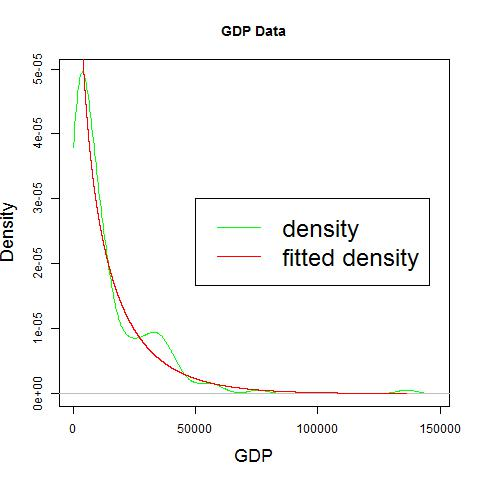
\includegraphics[width=10cm, height=10cm]{gdpfit}
\end{center}

\end{enumerate}

\bigskip
\bigskip
 %%%%%%%% Question 4 %%%%%%%%%
\begin{question}{3.4}For any random variable $X$, let $M_X(t) = \mathrm{E} \: \mathrm{e}^{X(t)}$ and $S_X(t) = log(M_X(t))$. $M_X(t)$ is called 
the moment generating function and $SX(t)$ is the cumulant generating function. It is known that (Can you prove it? Not required.)

\begin{center}
$$
\frac{d}{dt} S_X(t) \Big|_{t=0} = \mathrm{E} \: X \;\;\; \text{ and} \;\;\; \frac{d^2}{dt^2} S_X(t) \Big|_{t=0} = Var(X) 
$$
\end{center}

Use this fact to answer the following questions.

\begin{enumerate}[(a)]

   \item Assume that $X$ follows a Gamma distribution with parameter $\alpha$ and $\beta$. Calculate the cumulant generating function of $\log (X)$;
   \item Calculate $ \mathrm{E} \: \log (X)$  and $Var(\log X)$. Write your final result by using the digamma function  $\psi (x) $
and trigamma function  $\psi_1 (x) $, where  $\psi (x) = (\log \Gamma(x))^{'}$ and  $\psi_1 (x) = (\log \Gamma(x)))^{''}$.
   \item Match the first and second moment of $\log(X)$, and derive the \texttt{MOM} estimator of $\alpha$ and $\beta$. \\*
(Hint: in \texttt{R}, you can use \texttt{digamma(x), trigamma(x),} and \\* \texttt{ limma::trigammaInverse(x).})

   \item Apply your estimator to the \texttt{GDP} dataset and estimate the parameters $\alpha$  and $\beta$.


\end{enumerate}


\end{question}

 \textbf{\color{TealBlue}\emph{Answer:} } 

Let $Y = \log (X)$ where  $X\sim\Gamma(\alpha,\beta)$.  
The distribution of $Y \sim $ \texttt{Log-of-Gamma}$(\alpha, \beta)$ is given by
$$
f_Y(y) = \frac{1}{\beta^\alpha \Gamma(\alpha)} \;\; \mathrm{e}^{\left(\alpha y - e^{y/\beta}\right)}\,1_{(-\infty,\infty)}(y)
$$


Before answering part (a), we first find the moment generating function of \texttt{Log-of-Gamma}$(\alpha, \beta)$.

\begin{center}
\subsubsection*{\color{TealBlue}\emph{Moment Generating Function of Log Of Gamma}}
\end{center}

We now find the Moment Generating Function (\texttt{MGF}) of \texttt{Log-Of-Gamma}$(\alpha, \beta)$. By definition:
$$
M_Y(t) = \int_{-\infty}^{+\infty} \mathrm{e}^{ty} \frac{1}{\beta^\alpha \Gamma(\alpha)} \;\; \mathrm{e}^{\left(\alpha y - e^{y/\beta}\right)} dy
$$
To integrate this we use an old trick: we try to leave inside the integral sign the part of the function that integrates to 1 (this is often an easily recognizeable \texttt{pdf}); we then pull the constants that get in the way of making this integral equal to 1 out of the integral sign. Luckily, this can be done here:
\begin{align*}
M_Y(t) &= \frac{1}{\beta^\alpha \; \Gamma(\alpha)} \int_{-\infty}^{+\infty} \mathrm{e}^{ty} \;\; \mathrm{e}^{\left(\alpha y - e^{y/\beta}\right)} dy\\
&= \frac{1}{\beta^\alpha \; \Gamma(\alpha)} \int_{-\infty}^{+\infty} \mathrm{e}^{\left(ty +\alpha y - e^{y/\beta}\right)} dy\\
&= \frac{1}{\beta^\alpha \; \Gamma(\alpha)} \cdot \frac{\beta^{\alpha + t} \; \Gamma(\alpha + t)}{\beta^{\alpha + t} \; \Gamma(\alpha + t)} \cdot \int_{-\infty}^{+\infty} \mathrm{e}^{\left(y(\alpha + t) - e^{y/\beta}\right)} dy\\
&= \frac{ \beta^{\alpha + t} \; \Gamma(\alpha + t) }{\beta^\alpha \; \Gamma(\alpha)}  \cdot \int_{-\infty}^{+\infty} \frac{1}{\beta^{t+\alpha} \; \Gamma(\alpha + t)} \mathrm{e}^{\left(y(\alpha + t) - e^{y/\beta}\right)} dy\\
&= \frac{\beta^t \; \Gamma(\alpha + t)}{\Gamma(\alpha)} 
\end{align*}
\\
\begin{enumerate}[(a)]

\item By definition, the cumulant generating function is simply:
$$
S_Y(t) = log(M_Y(t)) = log \left(\frac{\beta^t \; \Gamma(\alpha + t)}{\Gamma(\alpha)} \right)
$$
\item 
To find the expectation of \texttt{Log-Of-Gamma}, we differentiate $S_Y(t) = \log (M_Y(t))$ and evaluate the result at $t = 0$.

\begin{align*}
(S_Y(t))^{'} &= (\log (M_Y(t)))^{'} = \left(\log \left(\frac{\beta^t \; \Gamma(\alpha + t)}{\Gamma(\alpha)} \right)\right)^{'} \\
&= \frac{1}{\frac{\beta^t \; \Gamma(\alpha + t)} {\Gamma(\alpha)}} \cdot \frac{1}{\Gamma(\alpha)} \cdot \left(  \beta^t \: \Gamma(\alpha + t)  \right)^{'}\\
&= \frac{\Gamma(\alpha)}{\beta^t \; \Gamma(\alpha + t)}  \cdot \frac{1}{\Gamma(\alpha)} \cdot \left(  \beta^t \log(\beta) \; \Gamma(\alpha + t) + \beta^t \; \Gamma^{'} (\alpha +t) \right)\\
&= \log(\beta) + \frac{\Gamma^{'} (\alpha +t) }{\Gamma(\alpha + t)}\\
\end{align*}


The last term is the log-derivative of the Gamma function evaluated at $\alpha + t$. This log-derivative is called the \texttt{digamma} function and is denoted by $\psi(\cdot)$. Thus:
$$
(S_Y(t))^{'} =  \log(\beta) +\psi(\alpha +t)
$$

We \emph{conclude} that if $Y$ is \texttt{Log-Of-Gamma}$(\alpha, \beta)$ distributed, then its expectation is given by:
$$
 \boxed{\mathrm{E}\, Y =  \log(\beta) +\psi(\alpha)}
$$
To find the variance of $Y$, we we look at the second derivative, $(S_Y(t))^{''}$, and evaluate it at $t=0$.
\begin{align*}
(S_Y(t))^{''} &= (\log(\beta) +\psi(\alpha +t))^{'}\\
&= \psi^{'}(\alpha +t)
\end{align*}

The derivative of \texttt{digamma} is the so-called \texttt{trigamma} function:
%\begin{align*}
$$
\boxed{Var(Y) = \psi^{'}(\alpha) = \psi_1(\alpha) =  \text{\texttt{trigamma($\alpha$)}}}
$$
%\end{align*}

\item Now we use \texttt{limma::trigammaInverse()} to estimate $\alpha$. Since we estimate $Var(Y)$ by $m_2 - m_1^2$, our estimate of $\alpha$ is:
$$
\hat\alpha = \text{\texttt{limma::trigammaInverse}}(m_2 - m_1^2)
$$
And therefore our estimate for $\beta$ is 

\begin{align*}
\log(\hat\beta)= m_1 - \text{\texttt{digamma}}(\hat\alpha) \\
\end{align*}
or
\begin{align*}
\hat\beta = \mathrm{e}^{m_1 - \text{\texttt{digamma}}(\hat\alpha) }
\end{align*}

\item Applying the above results to our data, we get:

\begin{verbatim}
m1 <- mean(gdp)       # = 13478.52
m2 <- mean(gdp^2)     # = 460173780

new.alpha.hat <- limma::trigammaInverse(m2 - m1^2)   # = 5.992181e-05
new.log.of.beta <- m1 - digamma(new.alpha.hat)       # = 30167.52
new.beta.hat <- exp(m1 - digamma(new.alpha.hat))     # Inf
\end{verbatim}

\end{enumerate}

 \end{document}
%Note 1: The * tells LaTeX not to number the lines.  If you remove the *, be sure to remove it below, too.
%Note 2: Inside the  environment, you do not want to use $-signs.  The reason for this is that this is already a math environment. This is why we have to include \text{} around any text inside the align environment.

%\begin{proof}
%Blah, blah, blah.  
%\end{proof}































